\section{Plačiau apie vokselius}

\subsection{Vokselis}

Pradėkime nuo vokselio apibrėžimo:

{\bf Vokselis} -- tūrinis elementas, reprezentuojantis patį mažiausią galimą
diskretizuotos trimatės erdvės elementą.

Pakankamai paprastas apibrėžimas, bet galimi ir kitokie jo variantai:

Sukapokime stačiakampio gretasienio (gali būti ir kubas) aprėpiamą erdvę į
$LxNxM$ elementus. Visi tie maži stačiakampiukai gretasieniai ir bus
{\bf vokseliai}.

\begin{figure}
\centering
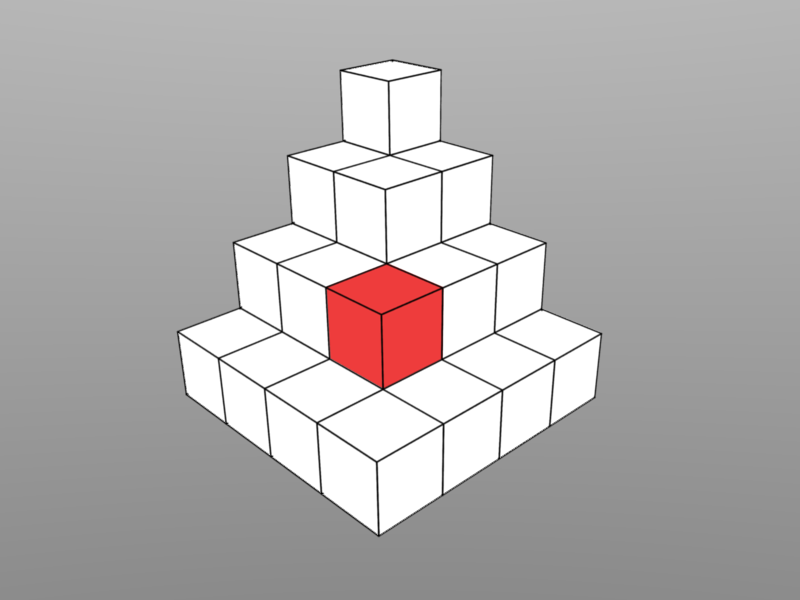
\includegraphics[height=6cm]{voxels.png}
\caption{Vokseliai (visi kubai) ir vokselis (raudonas kubas).}
\label{fig:voxels}
\end{figure}

Vokselis yra dvimačio objekto -- fragmento (su tam tikromis išlygomis galima
prilyginti pikseliui) praplėtimas trimatėje erdvėje. Kaip ir fragmento, taip
ir vokselio pagrindinė savybė yra jo pozicija. Tik vokseliai dar turi ir $Z$
koordinatę. Visos kitos vokselio savyje nešamos informacijos kiekis priklauso
nuo panaudojimo reikmių. Kaip ir fragmentų atveju, populiariausios yra $RGB$
ir $RGBA$ ($R$ -- \emph{red}, raudona; $G$ -- \emph{green}, žalia; $B$ --
\emph{blue}, mėlyna; $A$ -- \emph{alpha}, permatomumo) duomenų komponentės.
Kitaip nei fragmente, taip pat gana dažnai vokselis turi savo normalės
duomenis -- vis dėlto perlipama į trimatę erdvę.

To pačio vokselio interpretavimas, vėlgi, gana stipriai priklauso nuo tūrinui
vizualizavimui juos panaudojančios aplikacijos poreikių. Pavyzdžiui: Galima
laikyti, kad vokselių reikšmės yra „gry-nos“ tik jų centruose -- visur kitur
tūrio reikšmės yra interpoliuojamos tarp gretimų centrų reikšmių. Taip pat
galima laikyti, kad tūrinio objekto erdvės, kurią gaubia vokselis, įvairios
reikšmės (Pavyz-džiui $RGBA$) yra vienodos ir jas apibrėžia tas duotasis
vokselis.

\subsection{Panaudojimo sritys}

Visų pirma reiktų paminėti mokslinius įvairių sričių tyrimus. Medicina,
archeologija, biologija -- turbūt būtų plačiausiai tūrinį vizualizavimą
naudojančios mokslo sritys. Tūrinis vizualizavimas (o tuo pačiu ir vokselių
idėjos) jose dažniausiai naudojamos, vaizduojant įvairius duomenis.
Pavyzdžiui: kompiuterinės tomografijos, magnetinio rezonanso, ultragarso.
Moksle vokseliai naudojami, nes neretai ten būtina žinoti (ir matyti) visą
tūrinį objektą ir jį sudarančius vokselius -- o tam vien trimačių paviršių
neužtenka.

Žinoma, vien „rimtaisiais“ mokslais vizualizavimas neužsibaigia. Visa
volumetrikos idėja taip pat yra panaudojama tiesiog gražiems (priklauso nuo
skonio) vaizdams generuoti. Daugiausia vie-tos po saule vokseliai yra
išsikovoję vaizdo medžiagos specialiųjų efektų srityje.

Tuo tarpu viena iš plačiausiai trimatę grafiką naudojančių sričių --
kompiuteriniai žaidimai -- tūrinį vizualizavimą yra primiršę ir paprastai
išsiverčia tik su paviršių (poligonų) vizualizavimu. Bet populiarėjant
kompiuteriniams žaidimams ir vis gerėjant aparatūrinei įrangai, didės vis
kokybiškesnių ir kokybiškesnių realaus laiko kompiuterinės grafikos vaizdinių
poreikis. Tada žaidimų kūrėjai susidurs su tomis pačiomis problemomis, su
kuriomis jau susidūrė specialiųjų efektų studijos -- kai kurie efektai tiesiog
„nesižiūri“, naudojant vien tik paviršius. Tikėtina, kad tuo metu atsiras
hibridiniai (tiek vokselius, tiek poligonus) panaudojantys žaidimų varikliukai
(Industrijoje jau sklando kalbos, kad tokie varikliukai yra kuriami duotuoju
momentu).
